\subsection{Dynamical Systems}
%Requires Matrix Diagonalization and Markov Matrices 

The migration matrices discussed above give an example of a discrete
dynamical system. We call them discrete because they involve discrete values taken at a sequence of
points rather than on a continuous interval of time. 

An example of a situation
which can be studied in this way is a predator prey model. Consider the
following model where $x$ is the number of prey and $y$ the number of
predators in a certain area at a certain time. These are functions of $n\in \mathbb{N}$ where $n=1,2,\cdots $ are
the ends of intervals of time which may be of interest in the problem. In other words, $x \left( n \right)$ is the number 
of prey at the end of the $n^{th}$ interval of time.
An example of this situation may be modeled by the following equation
\begin{equation*}
\leftB
\begin{array}{c}
x\left( n+1\right) \\
y\left( n+1\right)
\end{array}
\rightB =\leftB
\begin{array}{rr}
2 & -3 \\
1 & 4
\end{array}
\rightB \leftB
\begin{array}{c}
x\left( n\right) \\
y\left( n\right)
\end{array}
\rightB
\end{equation*}
This says that from time period $n$ to $n+1$, $x$ increases if there are more $x$ and decreases as there
are more $y$. In the context of this example, this means that as the number of predators increases,
the number of prey decreases. As for $y,$ it increases if there are more $y$ and also if
there are more $x$.

This is an example of a matrix recurrence which we define now. 

\begin{definition}{Matrix Recurrence}{matrixrecurrence}
Suppose a dynamical system is given by  
\begin{eqnarray*}
x_{n+1} &=& a x_n + b y_n \\
y_{n+1} &=& c x_n + d y_n
\end{eqnarray*}

This system can be expressed as $V_{n+1} = A V_{n}$ where $V_{n} = \leftB \begin{array}{r}
x_n \\
y_n
\end{array}
\rightB$ and $A = \leftB \begin{array}{rr}
a & b \\
c & d 
\end{array} \rightB$.  
\end{definition}

In this section, we will examine how to find solutions to a dynamical system given certain initial conditions. This process involves several concepts previously studied, including matrix diagonalization and Markov matrices. The procedure is given as follows. Recall that when diagonalized, we can write $A^{n} = PD^{n}P^{-1}$. 

\begin{procedure}{Solving a Dynamical System}{solvingdynamical}
Suppose a dynamical system is given by  
\begin{eqnarray*}
x_{n+1} &=& a x_n + b y_n \\
y_{n+1} &=& c x_n + d y_n
\end{eqnarray*}

Given initial conditions $x_0$ and $y_0$, the solutions to the system are found as follows:
\begin{enumerate}
\item
Express the dynamical system in the form $V_{n+1} = AV_n$.
\item
Diagonalize $A$ to be written as $A = PDP^{-1}$.
\item 
Then $V_{n} = PD^{n} P^{-1} V_{0}$ where $V_{0}$ is the vector containing the initial conditions. 
\item
If given specific values for $n$, substitute into this equation. Otherwise, find a general solution for $n$.
\end{enumerate}
\end{procedure}

We will now consider an example in detail.

\begin{example}{Solutions of a Discrete Dynamical System}{solutionsdynamicalsystem}
Suppose a dynamical system is given by 
\begin{eqnarray*}
x_{n+1} &=& 1.5 x_n - 0.5y_n\\
y_{n+1} &=& 1.0 x_n
\end{eqnarray*}

Express this system as a matrix recurrence and find solutions to the dynamical system for initial conditions $x_0=20, y_0=10$. 
\end{example}

\begin{solution}
First, we express the system as a matrix recurrence. 
\begin{eqnarray*}
V_{n+1} &=& AV_{n}\\
\leftB
\begin{array}{c}
x\left( n+1\right) \\
y\left( n+1\right)
\end{array}
\rightB &=&\leftB 
\begin{array}{rr}
1.5 & -0.5 \\
1.0 & 0
\end{array}
\rightB \leftB
\begin{array}{c}
x\left( n\right) \\
y\left( n\right)
\end{array}
\rightB
\end{eqnarray*}

Then
\begin{equation*}
A
=
\leftB 
\begin{array}{rr}
1.5 & -0.5 \\
1.0 & 0
\end{array}
\rightB
\end{equation*}
You can verify that the eigenvalues of $A$ are $1$ and $.5$. By diagonalizing, we can write $A$ in the form
\begin{equation*}
P^{-1} D P =
\leftB
\begin{array}{rr}
1 & 1 \\
1 & 2
\end{array}
\rightB \leftB
\begin{array}{rr}
1 & 0 \\
0 & .5
\end{array}
\rightB \leftB
\begin{array}{rr}
2 & -1 \\
-1 & 1
\end{array}
\rightB
\end{equation*}

Now given an initial condition
\begin{equation*}
V_0 = \leftB
\begin{array}{c}
x_{0} \\
y_{0}
\end{array}
\rightB
\end{equation*}
the solution to the dynamical system is given by 
\begin{eqnarray*}
V_n &=& P D^n P^{-1} V_0\\
\leftB
\begin{array}{c}
x\left( n\right) \\
y\left( n\right)
\end{array}
\rightB &=&\leftB
\begin{array}{rr}
1 & 1 \\
1 & 2
\end{array}
\rightB \leftB
\begin{array}{rr}
1 & 0 \\
0 & .5
\end{array}
\rightB ^{n}\leftB
\begin{array}{rr}
2 & -1 \\
-1 & 1
\end{array}
\rightB \leftB
\begin{array}{c}
x_{0} \\
y_{0}
\end{array}
\rightB \\
&=&\leftB
\begin{array}{rr}
1 & 1 \\
1 & 2
\end{array}
\rightB \leftB
\begin{array}{rr}
1 & 0 \\
0 & \left( .5\right) ^{n}
\end{array}
\rightB \leftB
\begin{array}{rr}
2 & -1 \\
-1 & 1
\end{array}
\rightB \leftB
\begin{array}{c}
x_{0} \\
y_{0}
\end{array}
\rightB \\
&=&\leftB
\begin{array}{c}
y_{0}\left( \left( .5\right) ^{n}-1\right) -x_{0}\left( \left( .5\right)
^{n}-2\right) \\
y_{0}\left( 2\left( .5\right) ^{n}-1\right) -x_{0}\left( 2\left( .5\right)
^{n}-2\right)
\end{array}
\rightB 
\end{eqnarray*}

If we let $n$ become arbitrarily large, this vector approaches 
\begin{equation*}
\leftB
\begin{array}{c}
2x_{0}-y_{0} \\
2x_{0}-y_{0}
\end{array}
\rightB 
\end{equation*}

Thus for large $n,$
\begin{equation*}
\leftB
\begin{array}{c}
x\left( n\right) \\
y\left( n\right)
\end{array}
\rightB \approx \leftB
\begin{array}{c}
2x_{0}-y_{0} \\
2x_{0}-y_{0}
\end{array}
\rightB
\end{equation*}

Now suppose the initial condition is given by 
\begin{equation*}
\leftB
\begin{array}{c}
x_{0} \\
y_{0}
\end{array}
\rightB
=
\leftB
\begin{array}{r}
20 \\
10
\end{array}
\rightB
\end{equation*}

Then, we can find solutions for various values of $n$. Here are the
solutions for values of $n$ between $1$ and $5$
\begin{equation*}
n=1:
\leftB
\begin{array}{r}
25.0 \\
20.0
\end{array}
\rightB,
n=2: \leftB
\begin{array}{r}
27.5 \\
25.0
\end{array}
\rightB,
n=3: \leftB
\begin{array}{r}
28.75 \\
27.5
\end{array}
\rightB
\end{equation*}
\begin{equation*}
n=4: \leftB
\begin{array}{r}
29.375 \\
28.75
\end{array}
\rightB,
n=5: \leftB
\begin{array}{r}
29.688 \\
29.375
\end{array}
\rightB
\end{equation*}

Notice that as $n$ increases, we approach the vector given by  
\begin{equation*}
\leftB
\begin{array}{c}
2x_{0}-y_{0} \\
2x_{0}-y_{0}
\end{array}
\rightB
=
\leftB
\begin{array}{r}
2\left(20\right)- 10\\
2\left( 20 \right)-10
\end{array}
\rightB
=
\leftB
\begin{array}{r}
30\\
30
\end{array}
\rightB
\end{equation*}

These solutions are graphed in the following figure. 

\begin{center}
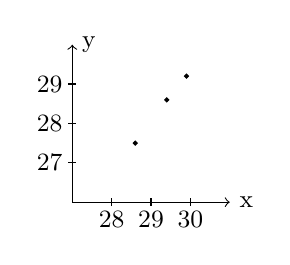
\begin{tikzpicture}[font=\small]
\draw[<->](0,2) --(0,0)--(2,0);
\draw (0.5, -0.05)--(0.5,0.05);
\draw (1, -0.05)--(1,0.05);
\draw (1.5, -0.05)--(1.5,0.05);
\draw (-0.05, 0.5)--(0.05,0.5);
\draw (-0.05, 1)--(0.05,1);
\draw (-0.05, 1.5)--(0.05,1.5);
\draw[fill] (0.8,0.75) circle [radius=0.025];
\draw[fill] (1.2,1.3) circle [radius=0.025];
\draw[fill] (1.45,1.6) circle [radius=0.025];
\node[right] at (2,0){x};
\node[right] at (0,2){y};
\node[below] at (0.5,0){$28$};
\node[below] at (1,0){$29$};
\node[below] at (1.5,0){$30$};
\node[left] at (0,0.5){$27$};
\node[left] at (0,1){$28$};
\node[left] at (0,1.5){$29$};
\end{tikzpicture}
\end{center}

\end{solution}

The following example demonstrates another system which exhibits some interesting behavior. When we graph 
the solutions, it is
possible for the ordered pairs to spiral around the origin.

\begin{example}{Finding Solutions to a Dynamical System}{findsolutionsdynamicalsystem}
Suppose a dynamical system is of the form
\begin{equation*}
\leftB
\begin{array}{c}
x\left( n+1\right) \\
y\left( n+1\right)
\end{array}
\rightB =\leftB 
\begin{array}{rr}
0.7 & 0.7 \\
-0.7 & 0.7
\end{array}
\rightB \leftB
\begin{array}{c}
x\left( n\right) \\
y\left( n\right)
\end{array}
\rightB
\end{equation*}
Find solutions to the dynamical system for given initial conditions.
\end{example}

\begin{solution}
Let
\begin{equation*}
A
=
\leftB 
\begin{array}{rr}
0.7 & 0.7 \\
-0.7 & 0.7
\end{array}
\rightB
\end{equation*}
To find solutions, we must diagonalize $A$. You can verify that the eigenvalues of $A$ are complex and are given by  $\lambda_1 = .7+.7i$ and $\lambda_2 = .7-.7i$. The eigenvector for $\lambda_1 = .7+.7i$ is 
\begin{equation*}
\leftB
\begin{array}{r}
1 \\
i
\end{array}
\rightB 
\end{equation*}
and that the eigenvector for $\lambda_2 = .7-.7i$ is
\begin{equation*}
\leftB
\begin{array}{r}
1 \\
-i
\end{array}
\rightB  
\end{equation*}

Thus the matrix $A$ can be written in the form
\begin{equation*}
\leftB
\begin{array}{rr}
1 & 1 \\
i & -i
\end{array}
\rightB \leftB
\begin{array}{cc}
.7+.7i & 0 \\
0 & .7-.7i
\end{array}
\rightB \leftB
\begin{array}{rr}
\vspace{0.05in}\frac{1}{2} & -\vspace{0.05in}\frac{1}{2}i \\
\vspace{0.05in}\frac{1}{2} & \vspace{0.05in}\frac{1}{2}i
\end{array}
\rightB
\end{equation*}
and so,
\begin{eqnarray*}
V_n &=& PD^nP^{-1}V_0 \\
\leftB
\begin{array}{c}
x\left( n\right) \\
y\left( n\right)
\end{array}
\rightB &=&\leftB
\begin{array}{rr}
1 & 1 \\
i & -i
\end{array}
\rightB \leftB
\begin{array}{cc}
\left( .7+.7i\right) ^{n} & 0 \\
0 & \left( .7-.7i\right) ^{n}
\end{array}
\rightB \leftB
\begin{array}{rr}
\vspace{0.05in}\frac{1}{2} & -\vspace{0.05in}\frac{1}{2}i \\
\vspace{0.05in}\frac{1}{2} & \vspace{0.05in}\frac{1}{2}i
\end{array}
\rightB \leftB
\begin{array}{c}
x_{0} \\
y_{0}
\end{array}
\rightB
\end{eqnarray*}

The explicit solution is given by
\begin{equation*}
\leftB
\begin{array}{c}
x_{0}\left( \vspace{0.05in}\frac{1}{2}\left( 0.7-0.7i \right) ^{n}+\vspace{0.05in}\frac{1}{2}
\left( 0.7+0.7i\right) ^{n}\right) + \allowbreak y_{0}\left( \vspace{0.05in}\frac{1}{2}
i\left( 0.7-0.7i\right) ^{n}-\frac{1}{2}i \left(
0.7+0.7i\right)  ^{n}\right) \\
y_{0}\left( \vspace{0.05in}\frac{1}{2} \left( 0.7-0.7i \right) ^{n}+\vspace{0.05in}\frac{1}{2}
\left( 0.7+0.7i\right) ^{n}\right) -  x_{0}\left( \vspace{0.05in}\frac{1}{2}
i\left( 0.7-0.7i\right) ^{n}-\vspace{0.05in}\frac{1}{2}i\left( 
0.7+0.7i\right) ^{n}\right)
\end{array}
\rightB
\end{equation*}

Suppose the initial condition is
\begin{equation*}
\leftB
\begin{array}{c}
x_{0} \\
y_{0}
\end{array}
\rightB =\leftB
\begin{array}{r}
10 \\
10
\end{array}
\rightB
\end{equation*}
Then one obtains the following sequence of values which are graphed below by
letting $n=1,2,\cdots ,20$

\begin{center}
\includegraphics[bb=0 0 800 800,scale=.2]{figures/4dec.eps}
\end{center}

In this picture, the dots are the values and the dashed line is to help to
picture what is happening.

These points are getting gradually closer to the origin, but they are
circling the origin in the clockwise direction as they do so. As $n$ increases,
the vector  $\leftB
\begin{array}{c}
x\left( n\right) \\
y\left( n\right)
\end{array}
\rightB$ approaches $ \leftB
\begin{array}{r}
0 \\
0
\end{array}
\rightB$
\end{solution}

This type of behavior along with complex eigenvalues is typical of the
deviations from an equilibrium point in the Lotka Volterra system of
differential equations which is a famous model for predator-prey
interactions. These differential equations are given by
\begin{eqnarray*}
x^{\prime } &=&x\left( a-by\right) \\
y^{\prime } &=&-y\left( c-dx\right)
\end{eqnarray*}
where $a,b,c,d$ are positive constants. For example, you might have $X$ be
the population of moose and $Y$ the population of wolves on an island.

Note that these equations make logical sense. The top says that the rate at which
the moose population increases would be $aX$ if there were no predators $Y$.
However, this is modified by multiplying instead by $\left( a-bY\right) $
because if there are predators, these will militate against the population
of moose.  The more predators there
are, the more pronounced is this effect. As to the predator equation, you
can see that the equations predict that if there are many prey around, then
the rate of growth of the predators would seem to be high. However, this is
modified by the term $-cY$ because if there are many predators, there would
be competition for the available food supply and this would tend to decrease
$Y^{\prime }.$

The behavior near an equilibrium point, which is a point where the right
side of the differential equations equals zero, is of great interest. In
this case, the equilibrium point is
\begin{equation*}
x=\frac{c}{d}, y=\frac{a}{b}
\end{equation*}
Then one defines new variables according to the formula
\begin{equation*}
x+\frac{c}{d}=x,\ y=y+\frac{a}{b}
\end{equation*}
In terms of these new variables, the differential equations become
\begin{eqnarray*}
x^{\prime } &=&\left( x+\frac{c}{d}\right) \left( a-b\left( y+\frac{a}{b}
\right) \right) \\
y^{\prime } &=&-\left( y+\frac{a}{b}\right) \left( c-d\left( x+\frac{c}{d}
\right) \right)
\end{eqnarray*}
Multiplying out the right sides yields
\begin{eqnarray*}
x^{\prime } &=&-bxy-b\frac{c}{d}y \\
y^{\prime } &=&dxy+\frac{a}{b}dx
\end{eqnarray*}
The interest is for $x,y$ small and so these equations are essentially equal
to
\begin{equation*}
x^{\prime }=-b\frac{c}{d}y,\ y^{\prime }=\frac{a}{b}dx
\end{equation*}

Replace $x^{\prime }$ with the difference quotient $\frac{x\left( t+h\right)
-x\left( t\right) }{h}$ where $h$ is a small positive number and $y^{\prime
} $ with a similar difference quotient. For example one could have $h$
correspond to one day or even one hour. Thus, for $h$ small enough, the
following would seem to be a good approximation to the differential
equations.
\begin{eqnarray*}
x\left( t+h\right) &=&x\left( t\right) -hb\frac{c}{d}y \\
y\left( t+h\right) &=&y\left( t\right) +h\frac{a}{b}dx
\end{eqnarray*}
Let $1,2,3,\cdots $ denote the ends of discrete intervals of time having
length $h$ chosen above. Then the above equations take the form
\begin{equation*}
\leftB
\begin{array}{c}
x\left( n+1\right) \\
y\left( n+1\right)
\end{array}
\rightB =\leftB
\begin{array}{cc}
1 & -\vspace{0.05in}\frac{hbc}{d} \\
\vspace{0.05in}\frac{had}{b} & 1
\end{array}
\rightB \leftB
\begin{array}{c}
x\left( n\right) \\
y\left( n\right)
\end{array}
\rightB
\end{equation*}
Note that the eigenvalues of this matrix are always complex.

We are not interested in time intervals of length $h$ for $h$ very small.
Instead, we are interested in much longer lengths of time. Thus, replacing
the time interval with $mh,$
\begin{equation*}
\leftB
\begin{array}{c}
x\left( n+m\right) \\
y\left( n+m\right)
\end{array}
\rightB =\leftB
\begin{array}{cc}
1 & -\vspace{0.05in}\frac{hbc}{d} \\
\vspace{0.05in}\frac{had}{b} & 1
\end{array}
\rightB ^{m}\leftB
\begin{array}{c}
x\left( n\right) \\
y\left( n\right)
\end{array}
\rightB
\end{equation*}
For example, if $m=2,$ you would have
\begin{equation*}
\leftB
\begin{array}{c}
x\left( n+2\right) \\
y\left( n+2\right)
\end{array}
\rightB =\leftB
\begin{array}{cc}
1-ach^{2} & -2b\vspace{0.05in}\frac{c}{d}h \\
2\vspace{0.05in}\frac{a}{b}dh & 1-ach^{2}
\end{array}
\rightB \leftB
\begin{array}{c}
x\left( n\right) \\
y\left( n\right)
\end{array}
\rightB
\end{equation*}
Note that most of the time, the eigenvalues of the new matrix will be complex.

You can also notice that the upper right corner will be negative by
considering higher powers of the matrix. Thus letting $1,2,3,\cdots $ denote
the ends of discrete intervals of time, the desired discrete dynamical
system is of the form
\begin{equation*}
\leftB
\begin{array}{c}
x\left( n+1\right) \\
y\left( n+1\right)
\end{array}
\rightB =\leftB
\begin{array}{rr}
a & -b \\
c & d
\end{array}
\rightB \leftB
\begin{array}{c}
x\left( n\right) \\
y\left( n\right)
\end{array}
\rightB
\end{equation*}
where $a,b,c,d$ are positive constants and the matrix will likely have
complex eigenvalues because it is a power of a matrix which has complex
eigenvalues.

You can see from the above discussion that if the eigenvalues of the matrix
used to define the dynamical system are less than 1 in absolute value, then
the origin is stable in the sense that as $n\rightarrow \infty ,$ the
solution converges to the origin. If either eigenvalue is larger than 1 in
absolute value, then the solutions to the dynamical system will usually be
unbounded, unless the initial condition is chosen very carefully. The next
example exhibits the case where one eigenvalue is larger than 1 and the
other is smaller than 1.

The following example demonstrates a familiar concept as a dynamical system.

\begin{example}{The Fibonacci Sequence}{fibonacci}
The Fibonacci sequence is the sequence given by 
\begin{equation*}
1, 1, 2, 3, 5, \cdots
\end{equation*}
which is defined recursively in the
form
\begin{equation*}
x\left( 0\right) =1=x\left( 1\right) ,\ x\left( n+2\right) =x\left(
n+1\right) +x\left( n\right)
\end{equation*}
Show how the Fibonacci Sequence can be considered a dynamical system.
\end{example}

\begin{solution}
This sequence is extremely important in the study of reproducing rabbits. It
can be considered as a dynamical system as follows. Let $y\left( n\right)
=x\left( n+1\right) .$ Then the above recurrence relation can be written as
\begin{equation*}
\leftB
\begin{array}{c}
x\left( n+1\right) \\
y\left( n+1\right)
\end{array}
\rightB =\leftB
\begin{array}{rr}
0 & 1 \\
1 & 1
\end{array}
\rightB \leftB
\begin{array}{c}
x\left( n\right) \\
y\left( n\right)
\end{array}
\rightB ,\ \leftB
\begin{array}{c}
x\left( 0\right) \\
y\left( 0\right)
\end{array}
\rightB =\leftB
\begin{array}{r}
1 \\
1
\end{array}
\rightB
\end{equation*}

Let 
\begin{equation*}
A
=
\leftB
\begin{array}{rr}
0 & 1 \\
1 & 1
\end{array}
\rightB
\end{equation*}

The eigenvalues of the matrix $A$ are $\lambda_1 = \frac{1}{2}-\frac{1}{2}\sqrt{5}$ and 
$\lambda_2 = \frac{1}{2}\sqrt{5}+\frac{1}{2}$. The corresponding eigenvectors are, respectively,
\begin{equation*}
X_1 = 
\leftB
\begin{array}{c}
-\vspace{0.05in}\frac{1}{2}\sqrt{5}-\vspace{0.05in}\frac{1}{2} \\
1
\end{array}
\rightB ,
X_2 = \leftB
\begin{array}{c}
\vspace{0.05in}\frac{1}{2}\sqrt{5}-\vspace{0.05in}\frac{1}{2} \\
1
\end{array}
\rightB 
\end{equation*}

You can see from a short computation that one of the eigenvalues is smaller than 1 in
absolute value while the other is larger than 1 in absolute value.
Now, diagonalizing $A$ gives us 
\begin{equation*}
\leftB
\begin{array}{cc}
\vspace{0.05in}\frac{1}{2}\sqrt{5}-\vspace{0.05in}\frac{1}{2} & -\vspace{0.05in}\frac{1}{2}\sqrt{5}-\vspace{0.05in}\frac{1}{2} \\
1 & 1
\end{array}
\rightB ^{-1}\leftB
\begin{array}{rr}
0 & 1 \\
1 & 1
\end{array}
\rightB \leftB
\begin{array}{cc}
\vspace{0.05in}\frac{1}{2}\sqrt{5}-\vspace{0.05in}\frac{1}{2} & -\vspace{0.05in}\frac{1}{2}\sqrt{5}-\vspace{0.05in}\frac{1}{2} \\
1 & 1
\end{array}
\rightB
\end{equation*}
\begin{equation*}
=\leftB
\begin{array}{cc}
\vspace{0.05in}\frac{1}{2}\sqrt{5}+\vspace{0.05in}\frac{1}{2} & 0 \\
0 & \vspace{0.05in}\frac{1}{2}-\vspace{0.05in}\frac{1}{2}\sqrt{5}
\end{array}
\rightB 
\end{equation*}

Then it follows that for a given initial condition, the solution to this
dynamical system is of the form
\begin{eqnarray*}
\leftB
\begin{array}{c}
x\left( n\right) \\
y\left( n\right)
\end{array}
\rightB &=&\leftB
\begin{array}{cc}
\vspace{0.05in}\frac{1}{2}\sqrt{5}-\vspace{0.05in}\frac{1}{2} & -\vspace{0.05in}\frac{1}{2}\sqrt{5}-\vspace{0.05in}\frac{1}{2} \\
1 & 1
\end{array}
\rightB \leftB
\begin{array}{cc}
\left( \vspace{0.05in}\frac{1}{2}\sqrt{5}+\vspace{0.05in}\frac{1}{2}\right) ^{n} & 0 \\
0 & \left( \vspace{0.05in}\frac{1}{2}-\vspace{0.05in}\frac{1}{2}\sqrt{5}\right) ^{n}
\end{array}
\rightB \cdot \\
&&\leftB
\begin{array}{cc}
\vspace{0.05in}\frac{1}{5}\sqrt{5} & \vspace{0.05in}\frac{1}{10}\sqrt{5}+\vspace{0.05in}\frac{1}{2} \\
-\vspace{0.05in}\frac{1}{5}\sqrt{5} & \vspace{0.05in}\frac{1}{5}\sqrt{5}\left( \vspace{0.05in}\frac{1}{2}\sqrt{5}-\vspace{0.05in}\frac{1
}{2}\right)
\end{array}
\rightB \leftB
\begin{array}{r}
1 \\
1
\end{array}
\rightB
\end{eqnarray*}
It follows that
\begin{equation*}
x\left( n\right) =\left( \frac{1}{2}\sqrt{5}+\frac{1}{2}\right) ^{n}\left(
\frac{1}{10}\sqrt{5}+\frac{1}{2}\right) +\left( \frac{1}{2}-\frac{1}{2}\sqrt{%
5}\right) ^{n}\left( \frac{1}{2}-\frac{1}{10}\sqrt{5}\right)
\end{equation*}
\end{solution}

Here is a picture of
the ordered pairs $\left( x\left( n\right) ,y\left( n\right) \right) $ for $
n=0,1,\cdots ,n$.

\begin{center}
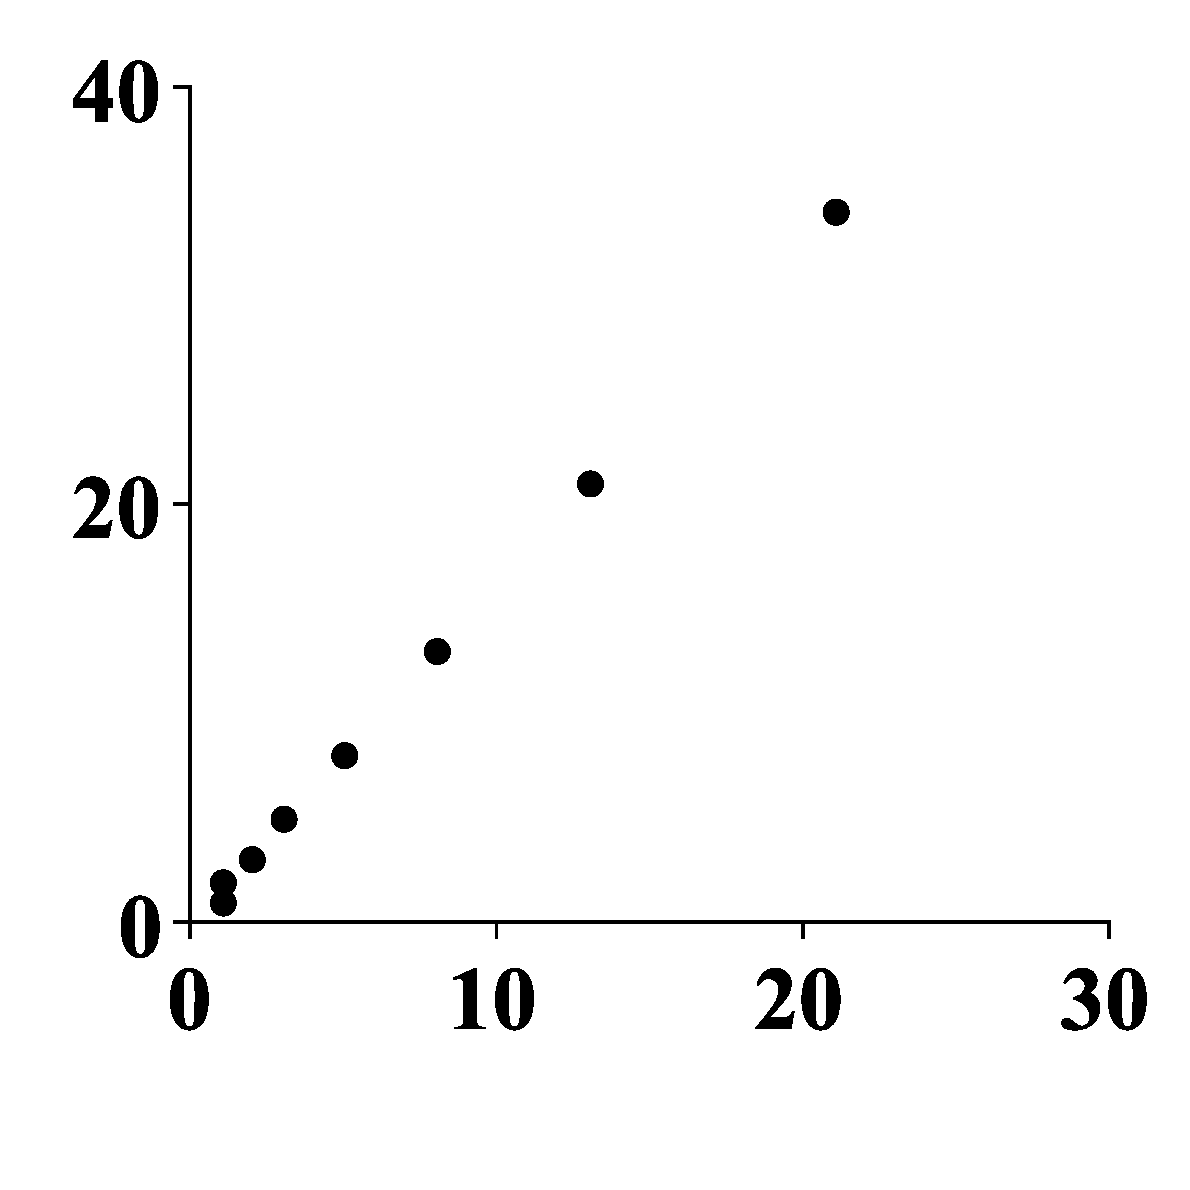
\includegraphics[bb=0 0 800 800,scale=.2]{figures/fibonacci.eps}
\end{center}

There is so much more that can be said about dynamical systems. It is a
major topic of study in differential equations and what is given above is
just an introduction.